%!TEX root = ../notes.tex
\section{May 3, 2022}
\subsection{Minkowski, Lagrange, and Waring Walk Into a Bar\dots}
\subsubsection{Four Squares Theorem and Waring's Problem}
\begin{theorem}[Lagrange, 1770]
    Every nonnegative integer can be written as a sum of four square integers.
\end{theorem}
In the same year, Waring asserted, in his book, that
\begin{theorem}[Waring, 1770]
    For every integer $k\geq 2$, there is a $g(k)$ such that every nonnegative integer can be written as a sum of at most $g(k)$ $k$th powers.
\end{theorem}
He claimed that $g(3) = 9$ and $g(4) = 19$. We note that $23$ and $239$ require $9$ cubes, and $79$ requires $19$ fourth powers. $g(3) = 9$ is a result of Wieferich-Kemper (1909) and $g(4) = 19$ is a result of Balasubramanian, Dress, Deshouillers (1986). Hilbert proved this theorem in $1909$.

There is also a `capital $G$' version of this question, which is an asymptotic best bound of $g(k)$.

$4 \leq G(3) \leq 7$. This is currently unknown.

$G(4) = 16$, which we do know. So, your mileage may very much vary on these.

\subsubsection{Lattices and Minkowski's Theorem}
\begin{definition}[Lattice]
    Let $e_1, e_2, \dots, e_n$ be a set of basis vectors for $\RR^n$. Then the additive subgroup of $(\RR^n, +)$ generated by $e_1, e_2, \dots, e_n$ is called a \ul{lattice}.
\end{definition}
\begin{example}
    The most obvious lattice in $\RR^n$ is $\ZZ^n$, where we take $e_i$ to be the standard basis vectors.

    We can take $\alpha\ZZ^n$ by some $0\neq \alpha\in\RR$ is also an obvious lattice.

    We can also take things like $\frac{1}{2}\ZZ\times \ZZ\subseteq\RR^2$.
\end{example}

\begin{definition}[Fundamental Domain]
    If $L$ is a lattice generated by $e_1, e_2, \dots, e_n$ in $\RR^n$, then the \ul{fundamental domain} of $L$ is the set
    \[\left\{ \sum a_i e_i \mid a_i\in\RR, 0\leq a_i < 1 \right\}\]
\end{definition}
\begin{example}
    If we take $\ZZ^2\subseteq\RR^2$, then the fundamental domain is the square with corners $(0, 0)$ to $(1, 1)$, with some dotted lines.
\end{example}
\begin{definition}[Convex, Symmetric]
    A set $X\subseteq\RR^n$ is \ul{convex} if forall $x, y\in X$,
    \[\lambda x + (1 - \lambda)y \in X\]
    for all $0\leq \lambda \leq 1$.

    A set $X$ is \ul{symmetric} if $x\in X$ implies $-x\in X$.
\end{definition}
\begin{example}
    *** A triangle is convex but not symmetric. An ellipse about the origin is convex and symmetric. An annulus is symmetric but not convex.
\end{example}
\begin{theorem}[Minkowski, p.140 \cite{stewart2015algebraic}]
    Let $L$ be an $n$-dimensional lattice in $\RR^n$ with fundamental domain $T$, and let $X$ be a bounded symmetric convex subset of $\RR^n$. If
    \[\Vol(X) > 2^n\Vol(T)\]
    then $X$ contains a non-zero point of $L$.
\end{theorem}
\begin{example}
    If we have
    ***
    \begin{center}
        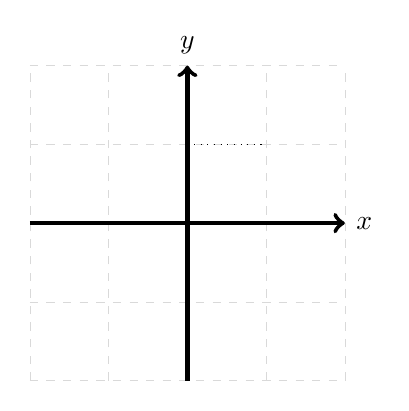
\begin{tikzpicture}
            \draw[help lines, color=gray!30, dashed] (-2,-2) grid (2,2);
            \draw[->,ultra thick] (-2,0)--(2,0) node[right]{$x$};
            \draw[->,ultra thick] (0,-2)--(0,2) node[above]{$y$};
            \draw[-, dotted] (0,1)--(1,1);
        \end{tikzpicture}
    \end{center}
    the $\ZZ^2$ example, if we have a `dotted' open square with area $4$, we just about not contain any nonzero points. If we add anything in, we'll have a nontrivial point.
\end{example}

\begin{proof}[Proof of 4 squares theorem using Minkowski's Theorem]
    We first prove this statement for primes, then extend to all positive integers. We first have
    \[2 = 1^2 + 1^2 + 0^2 + 0^2.\]
    So suppose we're trying to prove $p\in\ZZ_+$ is an odd prime.
    \begin{claim*}
        The equation $r^2 + s^2 + 1\equiv 0\pmod{p}$ has a solution $(r, s)\in\ZZ^2$.
    \end{claim*}
    \emph{Why?} Every element of $\ZZ/p\ZZ$ is a sum of $2$ squares\dots

    So let us select such an $r, s$. Consider the lattice $\Lambda\subseteq\ZZ^4$ that is given by
    \[\Lambda = A\ZZ^4,\]
    where
    \[A = \begin{pmatrix}
            p & 0 & r & s  \\
            0 & p & s & -r \\
            0 & 0 & 1 & 0  \\
            0 & 0 & 0 & 1
        \end{pmatrix}.\]
    We make an observation of the particular nature of the points in this lattice.

    If $\bvec{t}= (t_1, t_2, t_3, t_4)\in\ZZ^4$, and $\bvec{x} = (x_1, x_2, x_3, x_4)$ where $\bvec{x} = A\bvec{t}$, then
    \begin{align*}
        x_1^2 + x_2^2 + x_3^2 + x_4^2
         & = (pt_1 + rt_3 + st_4)^2 + (pt_2 + st_3 - rt_4)^2 + t_3^2 + t_4^2 \\
         & \equiv (rt_3 + st_4)^2 + (st_3 - rt_4)^2 + t_3^2 + t_4^2\pmod{p}  \\
         & = (1 + r^2 + s^2)(t_3^2 + t_4^2)\pmod{p}                          \\
         & = 0\pmod{p}
    \end{align*}
    Geometrically, the idea is if we can get the norm to be small enough, we know the sum is exactly $p$.

    Let's find an appropriate radius for our ball. A $4$-dimensional ball of radius $R$ has volume
    \[\pi^2R^4/2\]
    choose $R$ such that
    \begin{align*}
        16p^2 & < \frac{\pi^2 R^4}{2}\approx 4.93 R^4 \\
        4p    & < \approx 2.22 R^2                    \\
        2p    & < \approx 1.11 R^2
    \end{align*}
    The next condition is $R^2 < 2p$. So we want $R$ such that
    \[R^2 < 2p < \approx 1.11 R^2\]
    If we take $R^2 = 1.9p$ works.

    Let $X$ be the ball centered at the origin with radius $\sqrt{1.9p}$. Let $T$ be the fundamental domain for $\Lambda = A\ZZ^4$. Then we have $\Vol(T) = \det(A) = p^2$.

    Then $\Vol(X) > 2^n\Vol(T) = 16p^2$. Applying Minkowski's theorem, we conclude that $X$ \emph{must} contain some nonzero lattice point of $\Lambda$.

    If we let $\bvec{x} = (x_1, x_2, x_3, x_4)$ be this point. Then since $\bvec{x}\in X$, so
    \[x_1^2 + x_2^2 + x_3^2 + x_4^2 < R^2 < 2p.\]
    so $p\mid x_1^2 + x_2^2 + x_3^2 + x_4^2$ and $x_1^2 + x_2^2 + x_3^2 + x_4^2 < 2p$, and it's a nonzero point, so this forces
    \[x_1^2 + x_2^2 + x_3^2 + x_4^2 = p,\]
    which is as desired for primes.

    In the arbitrary case for arbitrary $n$, note that
    \begin{align*}
         & (a^2 + b^2 + c^2 + d^2)(A^2 + B^2 + c^2 + D^2)                \\
         & = (aA - bB - cC - dD)^2 + (aB + bA + cD - dC)^2 +             \\
         & \phantom{=}\ \ (aC - bD + cA + dB)^2 + (aD + bC - cB + dA)^2.
    \end{align*}
    so composite $n$ is also a sum of 2 squares.
\end{proof}

\begin{center}
    \emph{\dots and that's the course! }
\end{center}
